\documentclass[12pt,a4paper]{report}
\usepackage[utf8]{vietnam}
\usepackage{amsmath}
\usepackage{amsfonts}
\usepackage{amssymb}
\usepackage{makeidx}
\usepackage{graphicx}
\usepackage{fancybox}
\usepackage[left=3.50cm, right=2.00cm, top=3.50cm, bottom=3.00cm]{geometry}
\renewcommand{\baselinestretch}{1.5}
\usepackage{scrextend}
\changefontsizes{13pt}
\usepackage{fancyhdr}
\pagestyle{fancy}
\lhead{\textit{Đồ án tốt nghiệp đại học}}
\chead{}
\rhead{\textit{GVHD:PGS.TS Đỗ Đức Thuận}}
\lfoot{\textit{SVTH: Hoàng Thanh Lưu}}
\cfoot{\thepage}
\rfoot{\textit{Toán Tin K61}}
\renewcommand{\headrulewidth}{0.4pt}
\renewcommand{\footrulewidth}{0.4pt}
\begin{document}
	\thisfancypage{%đóng khung trang này
		\setlength{\fboxsep}{0pt}% 8pt là độ dày của đường viền
		\fbox}{} % phần nội dung sau là tương tự như đã làm
	\thispagestyle{empty}
	\begin{center}
		\vspace*{0cm}
		\fontsize{14}{12}
		\textbf{TRƯỜNG ĐẠI HỌC BÁCH KHOA HÀ NỘI}\\
		\textbf{VIỆN TOÁN ỨNG DỤNG VÀ TIN HỌC}\\
		\textbf{------ o0o ------}
	\end{center}
	\vspace*{0.4cm}
	\begin{figure}[h]
		\centering
		
\includegraphics[scale=.55]{./image/logo.png}
	\end{figure}
	\vspace*{0.4cm}
	\begin{center}
		\fontsize{20}{18}
		\textbf{ĐIỀU KHIỂN TỐI ƯU CHUYỂN ĐỘNG THẲNG CỦA TÊN LỬA}\\
		\vspace*{1.2cm}
		\fontsize{18}{16}
		\textbf{ĐỒ ÁN TỐT NGHIỆP ĐẠI HỌC}\\
		\fontsize{14}{16}
		\vspace*{0.4cm}
		\textit{Chuyên ngành:} \textbf{Toán Tin}
	\end{center}
	\vspace*{0.7cm}
	\begin{center}
		\fontsize{14}{16}
		\begin{tabular}{ll}
			
			\textbf{Giảng viên hướng dẫn:} & \textbf{PGS.TS ĐỖ ĐỨC THUẬN } \\ 
			\textbf{Sinh viên thực hiện:} & \textbf{HOÀNG THANH LƯU} \\ 
			\textbf{Lớp:}  & \textbf{TOÁN TIN K61} \\ 
		\end{tabular} \\
		\vspace*{1.6cm}
		\fontsize{14}{16}
		\textbf{Hà Nội - 12/2020}
	\end{center}
	\newpage
	\thispagestyle{empty}
	
	\chapter*{Lời nói đầu}
	\pagenumbering{arabic}
	\setcounter{page}{1}
	\textbf{Lý do chọn đề tài}\\\\
	Khi phải thiết kế, xây dựng bất kì một hệ thống điều khiển nào đó, các nhà thiết kế thường gặp phải bài toán thiết kế làm sao cho hệ thống đạt được chất lượng làm việc mong muốn như: tính ổn định, mức tiêu hao năng lượng thấp, tính bền vững cao...\\\\ Điều khiển tối ưu là một phần mở rộng của phép tính biến phân, là một phương pháp tối ưu hóa cho các lý thuyết điều khiển phát sinh.Điều khiển tối ưu có thể được xem như là một phương án điều khiển trong lý thuyết điều khiển tự dộng.\\\\
	\textbf{Đối tượng và phạm vi nghiên cứu} \\\\
	Đồ án đi sâu vào nghiên cứu cụ thể một số bài toán trong điều khiển tối ưu như:
	\begin{itemize}
		\item Bài toán liên quan đến điều khiển tối ưu cho các trạng thái cuối cùng có ràng buộc
		\item Cách chứng minh và giải ví dụ về bài toán
	\end{itemize}
	\textbf{Phương pháp nghiên cứu}
	\begin{itemize}
		\item Nghiên cứu lý thuyết: Phân tích các công trình được công bố ở lĩnh vực liên quan, thông qua bài giảng giáo án trên lớp
		\item Nghiên cứu thực tiển
		\item Lấy ý kiến chuyên gia: Tham khảo ý kiến của thầy giáo trực tiếp hướng dẫn.
	\end{itemize}
	Em xin gửi lời cảm ơn sâu sắc đến thầy Đỗ Đức Thuận đã giúp đỡ em hoàn thiện được đề tài !
	
	\tableofcontents
	
	\chapter{Cơ sở lý thuyết}
	\section{Vector và ma trận}
	\subsection{Vector}
	Bộ $n$ số thực $(x_1, x_2, ..., x_n)$ được gọi là vector $n$ chiều. Thông thường người ta viết các vector $n$ chiều dưới dạng cột
	$ \begin{bmatrix}
		x_1\\x_2\\\vdots\\x_n
	\end{bmatrix}$. Các phép toán cộng hai vector và nhân hai vector được định nghĩa như sau: giả sử $x = \begin{bmatrix}
		x_1\\x_2 \\\vdots \\x_n
	\end{bmatrix}$, $y = \begin{bmatrix}
		y_1\\y_2 \\\vdots \\y_n
	\end{bmatrix}$ thì \begin{center}
		$x + y = \begin{bmatrix}
			x_1\\x_2\\\vdots\\x_n
		\end{bmatrix} + \begin{bmatrix}
			y_1\\y_2\\\vdots\\ y_n
		\end{bmatrix} = \begin{bmatrix}
			x_1+y_1\\x_2 + y_2\\\vdots\\x_n + y_n
		\end{bmatrix}$ ; $cx = \begin{bmatrix}
			cx_1\\cx_2\\\vdots\\cx_n
		\end{bmatrix}$
	\end{center} 
	Với hai phép toán này, tập hợp tất cả các vector $n$ chiều tạo thành không gian tuyến tính $n$ chiều $\mathbb{R}^n$.
	\subsection{Ma trận}
	Ma trận $A = (a_{ij})_{m \times n}$ là một bảng số hình chữ nhật $A_{m \times n} = \begin{bmatrix}
		a_{11}&a_{12}&\cdots&a_{1n}\\
		a_{21}&a_{22}&\cdots&a_{2n}\\
		\cdots&\cdots&\ddots&\cdots\\
		a_{m1}&a_{m2}&\cdots&a_{mn}
	\end{bmatrix}$.\\ Cộng hai ma trận và nhân ma trận với hằng số: Nếu $A = (a_{ij})_{m \times n}$ và $B = (b_{ij})_{m \times n}$ thì tổng $A + B$ là 
	$$\begin{bmatrix}
		a_{11}&\cdots&a_{1n}\\
		a_{21}&\cdots&a_{2n}\\
		\cdots&\ddots&\cdots\\
		a_{m1}&\cdots&a_{mn}
	\end{bmatrix} + \begin{bmatrix}
		b_{11}&\cdots&b_{1n}\\
		b_{21}&\cdots&b_{2n}\\
		\cdots&\ddots&\cdots\\
		b_{m1}&\cdots&b_{mn}\end{bmatrix} = \begin{bmatrix}
		a_{11} + b_{11}&\cdots&a_{1n} + b_{1n}\\
		a_{21} + b_{21}&\cdots&a_{2n} + b_{2n}\\
		\cdots&\ddots&\cdots\\
		a_{m1} + b_{m1}&\cdots&a_{mn} + b_{mn}
	\end{bmatrix}$$ \\Tích của hằng số  $c$ và $A$ là $cA = \begin{bmatrix}
		ca_{11}&ca_{12}&\cdots&ca_{1n}\\
		ca_{21}&ca_{22}&\cdots&ca_{2n}\\
		\cdots&\cdots&\ddots&\cdots\\
		ca_{m1}&ca_{m2}&\cdots&ca_{mn}
	\end{bmatrix} $.
	
	\section{Chuyển vị}
	Một toán tử quan trọng của ma trận hay vector là toán tử \textit{chuyển vị (transpose)}.\\\\
	Cho $A \in \mathbb{R}^{m \times n}$, ta nói $B \in \mathbb{R}^{n \times m}$ là chuyển vị của $A$ nếu $b_{ij} = a_{ij}$, $\forall 1 \leq i \leq n, 1 \leq j \leq m$.\\Một cách ngắn gọn, chuyển vị của một ma trận là một ma trận nhận được từ ma trận cũ thông qua phép phản xạ gương qua đường chéo chính của ma trận ban đầu. Toán tử chuyển vị thường được kí hiệu bởi chữ $T, t$ hoặc kí tự $\top$. Trong báo cáo này, chúng ta sẽ sử dụng chữ cái $T$. Ví dụ chuyển vị của một vector $x$ được kí hiệu $x^T$, chuyển vị của một ma trận $A$ được kí hiệu $A^T$. Cụ thể: $$x = 
	\begin{bmatrix}
		x_1\\x_2\\ \vdots\\x_n
	\end{bmatrix} \Rightarrow x^T = [x_1 \text{ } x_2 \text{ } ... \text{ } x_n] \text{ ; }  A = \begin{bmatrix}
		a_{11} &\cdots &a_{1n}\\	a_{21}&\cdots &a_{2n}\\\cdots & \ddots & \cdots\\a_{m1}&\cdots&a_{mn}
	\end{bmatrix} \Rightarrow A^T = \begin{bmatrix}
		a_{11} &\cdots &a_{m1}\\	a_{12} &\cdots &a_{m2}\\\cdots & \ddots & \cdots\\a_{1n}&\cdots&a_{mn}
	\end{bmatrix}$$
	\section{Phép nhân hai ma trận}
	\subsection{Định nghĩa}
	Cho hai ma trận $A \in \mathbb{R}^{m \times n}, B \in \mathbb{R}^{n \times p}$, tích của hai ma trận được ký hiệu là $C = AB \in \mathbb{R}^{m \times p}$, trong đó phần tử ở hàng thứ $i$, cột thứ $j$ của ma trận kết quả được tính bởi:
	\begin{equation}
		c_{ij} = \sum^{n}_{k=1} a_{ik}b_{kj}, \forall 1 \leq i \leq m, 1 \leq j \leq p
	\end{equation}
	Điều kiện để nhân được hai ma trận là số cột của ma trận thứ nhất phải bằng số hàng của ma trận thứ hai. Trong định nghĩa trên, chúng đều bằng $n$.
	\subsection{Tính chất của phép nhân hai ma trận}
	Một vài tính chất của phép nhân hai ma trận (giả sử kích thước của các ma trận là phù hợp để các phép nhân ma trận tồn tại):
	\begin{itemize}
		\item Phép nhân ma trận không có tính chất giao hoán. Thông thường (không phải luôn luôn), $AB \neq BA$. Thậm chí trong nhiều trường hợp, các phép tính này không tồn tại vì kích thước các ma trận lệch nhau.
		\item Phép nhân ma trận có tính chất kết hợp. $ABC = (AB)C = A(BC)$.
		\item Phép nhân ma trận có tính chất phân phối đối với phép cộng: $A(B + C) = AB + AC$.
		\item Chuyển vị của một tích bằng tích các chuyển vị theo thứ tự ngược lại. 
	\end{itemize}
	\noindent
	Phép nhân của một ma trận $A \in \mathbb{R}^{m \times n}$ với một vector $x \in \mathbb{R}^{n}$ là một vector $b \in \mathbb{R}^m$:
	\begin{equation}
		Ax = b \text{, với } b_i = A_{:,i}x
	\end{equation} trong đó $A_{:,i}$  là vector hàng thứ $i$ của $A$.
	%%%%%%%%%%%%%%%%%%%%%%%%%%%%%%%%%%%
	\section{Ma trận đơn vị và ma trận nghịch đảo}
	\subsection{Ma trận đơn vị}
	\textit{Đường chéo chính} của một ma trận là tập hợp các điểm có chỉ số hàng và chỉ số cột là như nhau. Cách định nghĩa này cũng có thể được định nghĩa cho một ma trận không vuông. Cụ thể, nếu $A \in \mathbb{R}^{m \times n}$ thì đường chéo chính của $A$ bao gồm \{$a_{11}, a_{12}, ..., a_{pp}$\}, trong đó $p = min(m,n)$.\\\\
	Một ma trận đơn vị bậc $n$ là một ma trận đặc biệt trong $\mathbb{R}^{n \times n}$ với các phần tử trên đường chéo chính bằng 1, các phần tử còn lại bằng 0. Ma trận đơn vị thường được kí hiệu $I$ \textit{(identity matrix)}. Nếu làm việc với nhiều ma trận đơn vị với bậc khác nhau, ta kí hiệu $I_n$ cho ma trận đơn vị bậc $n$. Dưới đây là ma trận đơn vị bậc 3 và bậc 4.
	\begin{center}
		$I_3 = \begin{bmatrix}
			1&0&0\\0&1&0\\0&0&1
		\end{bmatrix}$; $I_4 = \begin{bmatrix}
			1&0&0&0\\0&1&0&0\\0&0&1&0\\0&0&0&1
		\end{bmatrix}$
	\end{center}
	Ma trận đơn vị có tính chất đặc biệt trong phép nhân. Nếu $A \in \mathbb{R}^{m \times n}, B \in \mathbb{R}^{n \times m}$ và $I$ là ma trận đơn vị bậc $n$, ta có: $AI =A, IB = B$.\\Với mọi vector $x \in \mathbb{R}^n$, ta có $I_nx = x$.
	\subsection{Ma trận nghịch đảo}
	Cho một ma trận vuông $A \in \mathbb{R}^{n \times n}$, nếu tồn tại ma trận vuông $B \in \mathbb{R}^{n \times n}$ sao cho $AB = I_n$, thì ta nói $A$ là khả nghịch \textit{(invertible, nonsingular hoặc nondegenerate)}, và $B$ được gọi là ma trận nghịch đảo \textit{(inverse matrix)} của $A$. Nếu không tồn tại ma trận $B$, ta nói $A$ là ma trận không khả nghịch \textit{(singular hoặc degenerate)}.\\\\
	Nếu $A$ là khả nghịch, ma trận nghịch đảo của nó thường được kí hiệu là $A^{-1}$. Ta cũng có:
	\begin{equation}
		A^{-1}A = AA^{-1} = I
	\end{equation}
	Ma trận nghịch đảo thường được sử dụng để giải hệ phương trình tuyến tính. Giả sử rằng $A \in \mathbb{R}^{n \times n}$ là một ma trận khả nghịch và một vector $b \in \mathbb{R}^n$ bất kì. Khi đó phương trình \begin{equation}
		Ax = b
	\end{equation} có nghiệm duy nhất là $x = A^{-1}b$. Thật vậy, nhân bên trái cả hai vế của phương trình (1.4) với $A^{-1}$, ta có $Ax=b \Rightarrow A^{-1}Ax = A^{-1}b \Leftrightarrow x = A^{-1}b$.
	\\\\Nếu $A$ không khả nghịch, thậm chí không vuông, phương trình tuyến tính (1.4) có thể không có nghiệm hoặc có vô số nghiệm.\\\\
	Giả sử các ma trận vuông $A, B$ là khả nghịch, khi đó tích của chúng cũng khả nghịch, và $(AB)^{-1} = B^{-1}A^{-1}$. Quy tắc này cũng khá giống với cách tính ma trận chuyển vị của tích các ma trận.
	
	\section{Ma trận xác định dương}
	\subsection{Định nghĩa}
	Một ma trận đối xứng $A \in \mathbb{R}^{n \times n}$ được gọi là xác định dương nếu: $$x^TAx > 0, \forall x\in \mathbb{R}^n, x \neq 0$$
	Một ma trận đối xứng $A \in \mathbb{R}^{n \times n}$ được gọi là nửa xác định dương nếu: $$x^TAx \geq 0, \forall x\in \mathbb{R}^n, x \neq 0$$
	Ma trận xác định âm và nửa xác định âm cũng được định nghĩa tương tự.	
	\subsection{Tính chất}
	\begin{itemize}
		\item Mọi trị riêng của một ma trận xác định dương đều là một số thực dương.  Mọi trị riêng của một ma trận nửa xác định dương đều là không âm.\item Mọi ma trận xác định dương là khả nghịch.  Hơn nữa, định thức của nó là một số dương. Điều này suy ra trực tiếp từ tính chất 1, với lưu ý rằng định thức của một ma trận bằng tích tất cả các trị riêng của nó.
		\item Nếu $A$ là một ma trận nửa xác định dương thì $x^TAx = 0 \Leftrightarrow Ax = 0.$ \\Nếu $Ax = 0 \Rightarrow x^TAx = 0$ một cách hiển nhiên.\\ Nếu $x^TAx = 0$. Với vector $y \neq 0$ bất kì có cùng kích thước với $x$, xét hàm số sau đây $$f(\lambda) = (x+\lambda y)^TA(x+ \lambda y)$$ Hàm số này không âm với mọi $\lambda$ vì $A$ là một ma trận nửa xác định dương. Đây là một tam thức bậc hai của $\lambda$ $$f(\lambda) = y^TAy\lambda^2 + 2y^TAx\lambda + x^TAx = y^TAy\lambda^2 + 2y^TAx\lambda$$ Xét hai trường hợp: 
		\begin{itemize}
			\item $y^TAy = 0$. Khi đó $f(\lambda) = 2y^TAx\lambda \geq 0, \forall \lambda$ nếu và chỉ nếu $y^TAx = 0$
			\item $y^TAy > 0$. Khi đó tam thức bậc hai $f(\lambda) \geq 0, \forall \lambda$ nếu và chỉ nếu $\Delta' = (y^TAx)^2 \leq 0$ vì hệ số ứng với thành phần bậc hai bằng $y^TAy > 0.$ Điều này cũng đồng nghĩa với việc $y^TAx = 0$.
		\end{itemize}
		Tóm lại, $y^TAx = 0, \forall y \neq 0$. Điều này chỉ xảy ra nếu $Ax = 0$.
	\end{itemize}
	\section{Đạo hàm}
	\subsection{Đạo hàm của một hàm trả về một số vô hướng}
	Đạo hàm bậc nhất (first-order gradient) hay viết gọn là đạo hàm (gradient) của một hàm số $f(x): \mathbb{R}^n \rightarrow \mathbb{R}$ theo $x$ được định nghĩa là
	\begin{eqnarray}
		\nabla_xf(x) = \begin{bmatrix}
			\dfrac{\partial f(x)}{\partial x_1}\\\dfrac{\partial f(x)}{\partial x_2}\\ \vdots \\ \dfrac{\partial f(x)}{\partial x_n}
		\end{bmatrix} \in \mathbb{R}^n
	\end{eqnarray} trong đó $\dfrac{\partial f(x)}{\partial x_i}$ là đạo hàm riêng (partial derivative) của hàm số thành phần thứ $i$ của vector $x$. Đạo hàm này được lấy khi tất cả các biến, ngoài $x_i$, được giả sử là hằng số. Nếu không có thêm biến nào khác, $\nabla_xf(x)$ thường được viết gọn là $\nabla f(x)$. Đạo hàm của hàm số này là một vector có cùng chiều với vector đang được lấy đạo hàm. Tức vector được viết dưới dạng cột thì đạo hàm cũng được viết dưới dạng cột. \\\\ Đạo hàm bậc hai (second-order gradient) của hàm số trên còn được gọi là Hessian và được định nghĩa như sau, với $\mathbb{S}^n \in \mathbb{R}^{n \times n}$ là tập các ma trận vuông đối xứng bậc $n$.
	\begin{eqnarray}
		\nabla^2f(x) = \begin{bmatrix}
			\dfrac{\partial^2 f(x)}{\partial x^2_1}&\dfrac{\partial^2 f(x)}{\partial x_1\partial x_2}&\cdots&\dfrac{\partial^2 f(x)}{\partial x_1\partial x_n} \\ 	\dfrac{\partial^2 f(x)}{\partial x_2 \partial x_1}&\dfrac{\partial^2 f(x)}{\partial x^2_2}&\cdots&\dfrac{\partial^2 f(x)}{\partial x_2\partial x_n} \\ \vdots & \vdots& \ddots& \vdots \\ 	\dfrac{\partial^2 f(x)}{\partial x_n \partial x_1}&\dfrac{\partial^2 f(x)}{\partial x_n\partial x_2}&\cdots&\dfrac{\partial^2 f(x)}{\partial x^2_n}
		\end{bmatrix} \in \mathbb{S}^n
	\end{eqnarray}
	Đạo hàm của một hàm số $f(X): \mathbb{R}^{n \times m} \rightarrow \mathbb{R}$ theo ma trận $X$ được định nghĩa là \begin{eqnarray}
		\nabla f(X) = \begin{bmatrix}
			\dfrac{\partial f(X)}{\partial x_{11}}&\dfrac{\partial f(X)}{\partial x_{12}}&\cdots&\dfrac{\partial f(X)}{\partial x_{1m}} \\ 	\dfrac{\partial f(X)}{ \partial x_{21}}&\dfrac{\partial f(X)}{\partial x_{22}}&\cdots&\dfrac{\partial f(X)}{\partial x_{2m}} \\ \vdots & \vdots& \ddots& \vdots \\ 	\dfrac{\partial f(X)}{\partial x_{n1}}&\dfrac{\partial f(X)}{\partial x_{n2}}&\cdots&\dfrac{\partial f(X)}{\partial x_{nm}}
		\end{bmatrix} \in \mathbb{R}^{n \times m}
	\end{eqnarray} 
	Đạo hàm của hàm số $f: \mathbb{R}^{m \times n} \to \mathbb{R}$ là một ma trận trong $\mathbb{R}^{m \times n}, \forall m, n \in \mathbb{N}^*$. Cụ thể, để tính đạo hàm của một hàm $f: \mathbb{R}^{m \times n} \to \mathbb{R}$, ta tính đạo hàm riêng của hàm số đó theo từng thành phần của ma trận khi toàn bộ các thành phần khác được giả sử là hằng số. Tiếp theo, ta sắp xếp các đạo hàm riêng tính được theo đúng thứ tự trong ma trận.
	
	\subsection{Đạo hàm của hàm trả về một vector}
	Xét một hàm trả về vector với đầu vào là một số thực $v(x): \mathbb{R} \to \mathbb{R}^n$: \begin{eqnarray}
		v(x) = \begin{bmatrix}
			v_1(x)\\v_2(x)\\ \cdots \\ v_n(x)
		\end{bmatrix}
	\end{eqnarray} Đạo hàm của hàm số này theo $x$ là một vector hàng như sau: \begin{eqnarray}
		\nabla v(x) = \begin{bmatrix}
			\dfrac{\partial v_1(x)}{\partial x} & 	\dfrac{\partial v_2(x)}{\partial x} & \cdots & 	\dfrac{\partial v_n(x)}{\partial x}
		\end{bmatrix}
	\end{eqnarray} Đạo hàm bậc hai của hàm số này có dạng \begin{eqnarray}
		\nabla^2 v(x) = \begin{bmatrix}
			\dfrac{\partial^2 v_1(x)}{\partial x^2} & 	\dfrac{\partial^2 v_2(x)}{\partial x^2} & \cdots & 	\dfrac{\partial^2 v_n(x)}{\partial x^2}
		\end{bmatrix}
	\end{eqnarray}
	\subsection{Tính chất quan trọng của đạo hàm}
	\subsubsection{Quy tắc tích (Product rule)} Để cho tổng quát ta giả sử biến đầu vào là một ma trận. Giả sử rằng các hàm số có chiều phù hợp để các phép nhân thực hiện được. Ta có \begin{equation}
		\nabla\big(f(X)^Tg(X)\big) = (\nabla f(X))g(X) + (\nabla g(X))f(X)
	\end{equation} Biểu thức này giống như biểu thức mà chúng ta đã quen thuộc: $$(f(x)g(x))' = f'(x)g(x) + g'(x)f(x)$$ Chú ý rằng với tích của vector và ma trận, ta không được sử dụng tính chất giao hoán.\subsubsection{Quy tắc chuỗi (Chain rule)}
	Khi có các hàm hợp thì \begin{equation}
		\nabla_xg(f(X)) = (\nabla_xf)^T(\nabla_fg)
	\end{equation} Quy tắc này cũng giống quy tắc trong hàm một biến: $$(g(f(x)))' = f'(x)g'(f)$$ Một lưu ý nhỏ nhưng quan trọng khi làm việc với tích các ma trận là sự phù hợp về kích thước của các ma trận trong tích.
	
	\section{Hàm tuyến tính, hàm afin}
	Một hàm số $f(x)$ xác định trên $\mathbb{R}^n$ được gọi là tuyến tính nếu $$f(\alpha x^1 + \beta x^2) = \alpha f(x^1) + \beta f(x^2)$$ với mọi $x^1, x^2$ $\in$ $\mathbb{R}^n$ và với mọi $\alpha$, $\beta$ $\in \mathbb{R}$. Một hàm tuyến tính xác định trên $\mathbb{R}^n$ luôn có dạng $f(x) = \langle c, x \rangle$, trong đó vector $c \in \mathbb{R}^n$ cho trước. \\\\
	Hàm số có dạng $f(x) = \langle c, x \rangle + \lambda$, trong đó vector $c \in \mathbb{R}^n$ và $\lambda \in \mathbb{R}$ cho trước, được gọi là hàm afin hay hàm tuyến tính afin. Dễ thấy nếu $f(x)$ là afin thì $\forall x, y \in \mathbb{R}^n, \forall \alpha, \beta \in \mathbb{R}$ mà  $\alpha$ + $\beta$ = 1 ta có $$f(\alpha x + \beta y) = \alpha f(x) + \beta f(y)$$
	
	\section{Bài toán tối ưu}
	\subsection{Các khái niệm cơ bản}
	Bài toán tối ưu dạng tổng quát: \begin{eqnarray}
		x^* = \text{arg} \min_x f_0(x)\\\text{thỏa mãn: } f_i(x) \leq 0, \quad i = 1,2,...,m \nonumber\\h_j(x) = 0, \quad j = 1,2,..., p \nonumber
	\end{eqnarray}
	Phát biểu bằng lời: Tìm giá trị của biến $x$ để tối thiểu hàm $f_0(x)$ trong số những giá trị $x$ thỏa mãn các điều kiện ràng buộc. Ta có bảng khái niệm và ký hiệu của bài toán tối ưu được trình bày trong bảng dưới.
	\begin{center}
		\begin{tabular}{|c|l|l|}
			\hline
			\textbf{Ký hiệu}& \textbf{Ý nghĩa } \\
			\hline
			$x \in \mathbb{R}^n$ & biến tối ưu \\
			\hline
			$f_0: \mathbb{R}^n \to \mathbb{R}$ &hàm mục tiêu \\
			\hline
			$f_i(x) \leq 0$& bất đẳng thức ràng buộc \\
			\hline
			$f_i: \mathbb{R}^n \to \mathbb{R}$& hàm bất đẳng thức ràng buộc \\
			\hline
			$h_j(x) = 0$& đẳng thức ràng buộc \\
			\hline
			$h_j: \mathbb{R}^n \to \mathbb{R}$& hàm đẳng thức ràng buộc \\
			\hline
			$\mathcal{D} = \bigcap_{i=0}^m\text{dom}f_i \cap \bigcap_{j=1}^p\text{dom}h_j$& tập xác định\\
			\hline
		\end{tabular}
		
	\end{center}
	Ngoài ra:
	\begin{itemize}
		\item Khi $m = p = 0$ thì bài toán (1.13) được gọi là bài toán tối ưu không ràng buộc.
		\item $\mathcal{D}$ là tập xác định, tức giao của tất cả các tập xác định của mọi hàm số xuất hiện trong bài toán. Tập hợp các điểm thỏa mãn mọi điều kiện ràng buộc là một tập con của $\mathcal{D}$ được gọi là tập khả thi. Khi tập khả thi là một tập rỗng thì bài toán tối ưu (1.13) là bất khả thi. Một điểm nằm trong tập khả thi được gọi là điểm khả thi.
		\item Giá trị tối ưu của bài toán tối ưu được định nghĩa là $$p^* = \inf\{f_0(x)|f_i(x) \leq 0, i = 1, ..., m; h_j(x) = 0, j=1,..., p\}$$
		$p^*$ có thể nhận các giá trị $\pm \infty$. Nếu bài toán là bất khả thi, ta coi $p^* = + \infty$. Nếu hàm mục tiêu không bị chặn dưới, ta coi $p^* = -\infty$
	\end{itemize}
	\subsection{Điểm tối ưu và tối ưu địa phương}
	Một điểm $x^*$ được gọi là điểm tối ưu của bài toán (1.13) nếu $x^*$ là một điểm khả thi và $f_0(x^*) = p^*$. Tập hợp tất cả các điểm tối ưu được gọi là tập tối ưu. Nếu tập tối ưu khác rỗng, ta nói bài toán (1.13) giải được. Ngược lại, nếu tập tối ưu rỗng, ta nói giá trị tối ưu không thể đạt được.\\\\ \textit{Ví dụ:} Xét hàm mục tiêu $f(x) = \dfrac{1}{x}$ với ràng buộc $x>0$. Giá trị tối ưu của bài toán này là $p^* = 0$ nhưng tập tối ưu là một tập rỗng vì không có giá trị nào của $x$ để hàm mục tiêu đạt giá trị $p^*$. \\\\ Với hàm một biến, một điểm là cực tiểu/tối ưu địa phương của hàm số nếu tại đó hàm số đạt giá trị nhỏ nhất trong một  lân cận (vì lân cận này thuộc tập xác định của hàm số). Trong không gian một chiều, lân cận của một điểm được hiểu là tập các điểm cách điểm đó một khoảng rất nhỏ. Trong không gian nhiều chiều, ta gọi một điểm $x$ là tối ưu địa phương nếu  tồn tại một giá trị $R > 0$ sao cho 
	\begin{eqnarray}
		f_0(x) = \inf\{f_0(z)|f_i(z)\leq 0, i =1,..., m, h_j(z) = 0, j=1,..., p, ||z-x||_2 \leq R\} \nonumber
	\end{eqnarray}
	
	\chapter{Một số vấn đề về bài toán điều khiển tối ưu}
	\section{Dạng tổng quát của bài toán điều khiển tối ưu}
	Dạng tổng quát chung của bài toán điều khiển tối ưu
	\begin{itemize}
		\item[(1)] Có phương trình trạng thái là $$\dot{x} = f_i(t,x_1,\cdots,x_n,u_1,\cdots, u_m), \qquad i = 1, \cdots, n$$ hoặc dạng vector $$\dot{x}=f(t,x,u),$$ với $$x = \begin{bmatrix}
			x_1\\\vdots\\ x_n
		\end{bmatrix} \qquad \text{và} \qquad u = \begin{bmatrix}
			u_1 \\\vdots\\u_m
		\end{bmatrix}$$
	\item[(2)] Trạng thái đầu tiên $x(0) = x_0 \in \mathbb{R}^n$, và trạng thái cuối cùng $x_1 \in \mathbb{R}^n$ có thể có hoặc không được cung cấp.
	\item[(3)] Lớp $\Delta$ của các điều khiển được chấp nhận là tập tất cả các điều khiển $u$ trong giới hạn về vật lý của bài toán. Thông thường chúng ta được cung cấp một tập lồi, compact $\Omega$ $\subset$ $\mathbb{R}^m$ (tập giới hạn) và ta thấy \begin{equation}
		\Delta = \{u=(u_1,\cdots, u_m) \text{ : $u_i$ rời rạc liên tục và $u(t) \in \Omega$}\} \nonumber
	\end{equation}
\item[(4)] Hàm mục tiêu so sánh hiệu quả của các điều khiển khác nhau. Thông thường: $$C(u) = \int_{0}^{t_1}f_0(t,x(t),u(t))dt$$ với $f_0$ là một hàm thực, liên tục xác định và tích phân ở trên được hiểu là chúng ta lấy một điều khiển $u\in\Delta$, giải phương trình trạng thái và thu được $x$ tương ứng, tính $f_0$ như là một hàm số của $t$, và thực hiện tích phân. \\\\ Nếu trạng thái kết thúc cho trước (gọi là bài toán cố định) khi đó $x(t_1)=x_1$. Cụ thể nếu $f_0 \equiv$ 1 thì $C(u)=t$, và chúng ta có vấn đề tối thiểu thời gian. Nếu trạng thái kết thúc không được cho trước (gọi là bài toán tự do), khi đó $t_1$ là một thời gian cố định, và tích phân được thực hiện trong khoảng thời gian cố định [0, $t_1$]. Vấn đề tìm điều khiển tối ưu có thể được đưa ra: Tìm một điều khiển được chấp nhận $u^*$ làm tối thiểu hàm mục tiêu, tức là $$C(u^*) \leq C(u), \forall u \in \Delta$$ Khi đó $u^*$ được gọi là điều khiển tối ưu.
	\end{itemize} 

\section{Nguyên lý cực đại Pontryagin}
\subsubsection{Xét hệ điều khiển} \begin{eqnarray}
	\dot{x}=f(x,u), f: \mathbb{R}^n \times \mathbb{R}^m \to \mathbb{R}^n, f = (f_1,\cdots,f_n)^T, f_i: \mathbb{R}^n \times \mathbb{R}^m \to \mathbb{R}, i=1,...,n \nonumber
\end{eqnarray}
Một số lưu ý
\begin{itemize}
	\item $x(0)=0 \in \mathbb{R}^n$\\$x(t_1) = x_1$ cho trước thì bài toán là bài toán cố định\\$x(t_1)=x_1$ không cho trước thì bài toán là bài toán tự do
	\item $x\in\Delta$ là lớp điều khiển chấp nhận được, $x(t_1)\in\Omega\subset\mathbb{R}^m$
	\item Hàm tối ưu $$C(x) = \int_{0}^{t_1}f_0(x(t), u(t))dt \to \text{min}$$
\end{itemize}
\subsubsection{Xây dựng hàm Hamilton}
\begin{eqnarray}
	H(x, u, \varphi) = \varphi_0f_0(x, u) + \varphi_1f_1(x, u) + \cdots + \varphi_nf_n(x,u)
\end{eqnarray} trong đó $\varphi_0, \varphi_1,...,\varphi_n \in \mathbb{R}$.
\subsubsection{Viết lại hàm Halminton}
\begin{eqnarray}
	H(x,u,\varphi
	)=\varphi_0f_0(x,u)+\langle\varphi,f\rangle = \varphi_0f_0(x,u) + \varphi^Tf
\end{eqnarray} trong đó $\varphi=(\varphi_1,\cdots,\varphi_n)^T$.

\subsubsection{Định lý PMP}
Giả sử $u^*$ là điều khiển tối ưu tương ứng với quỹ đạo trạng thái tối ưu $x^*$. Khi đó tồn tại hàm $\varphi^*(t) = \big(\varphi_1^*(t), \cdots,\varphi_n^*(t)\big)^T$ với hệ số $\varphi_0^*$ thỏa mãn: \begin{itemize}
	\item[\textbf{(a)}] $\dot{x}^* = f(x^*,u^*)$
	\item[\textbf{(b)}] $\dot{\varphi}_i^* = \dfrac{-\partial H}{\partial x_i} = -\varphi
	_0^*\dfrac{\partial f_0}{\partial x_i}-\varphi_1^*\dfrac{\partial f_1}{\partial x_i} - \cdots
	-\varphi
	^*_n\dfrac{\partial f_n}{\partial x_i}$
	\item[\textbf{(c)}] $\varphi_0^*$ là không dương và $$H(x^*,u^*,\varphi^*) = \max_{v\in\Omega} H(x^*,v,\varphi
	^*) = M(x^*,\varphi^*)$$ Hơn nữa $M(x^*(t), \varphi^*(t))$ là hằng số với $0\leq t\leq t^*$.
\end{itemize}
\subsubsection{Chú ý} Nếu các hàm số $f_0,f$ khả vi liên tục thì không mất tổng quát ta có thể giả sử $\varphi
_0^*=-1$. Đối với bài toán tự do ($x^*(t^*) = x_1$ không cho trước) thì ta có thêm điều kiện hoành $\varphi
^*(t^*) = 0.$
\section{Tính điều khiển được và quan sát được}
\subsubsection{Xét hệ điều khiển được}
\begin{eqnarray}
	\begin{cases}
		\dot{x} = Ax + Bu \\ x(0) = x_0 \in \mathbb{R}^n, A \in \mathbb{R}^{n\times n}, B \in \mathbb{R}^{n\times m}\\u(t) \in \Omega \subset \mathbb{R}^m
	\end{cases}
\end{eqnarray}
Trạng thái $x_1$ được gọi là đạt được từ trạng thái $x_0$ trong thời gian $t_a$ cho hệ (1.3) có nghiệm $x(0)=x_0, x(1) = x_1$. Khi đó ta cũng gọi là $x_0$ có thể dịch chuyển được đến $x_1$ trong thời gian $t_a$.
\subsubsection{Điều khiển được} Hệ (1.3) được gọi là điều khiển được trong thời gian $T > 0$ nếu với mọi trạng thái ban đầu $x_0 \in$ $\mathbb{R}^n$ và trạng thái cuối cùng $x_1 \in \mathbb{R}^n$ thì $x_1$ có thể đạt được từ $x_0$  trong thời gian $T > 0.$
\\
Hệ (1.3) được gọi là điều khiển được nếu nó điều khiển được trong một thời gian $T > 0$ nào đó.
\subsubsection{Điều khiển được về không}
Hệ (1.3) được gọi là điều khiển được về không nếu với trạng thái ban đầu $x_0$ tồn tại một điều khiển và một thời điểm $T > 0$ sao cho $$x(t) = x_1=0$$ Ta định nghĩa ma trận Kalman: $$[A|B] = [B, AB, \cdots, A^{n-1}B] \in \mathbb{R}^{n\times m}$$
\textbf{Định lý.} Hệ (1.3) là điều khiển được khi và chỉ khi $rank [A|B] = n$ (hệ không có ràng buộc, $\Omega = \mathbb{R}^n$).\\ Với hệ có ràng buộc ($\Omega$ $\subset$ $\mathbb{R}^n$). Giả sử 0 là phần trong của $\Omega$, hệ (1.3) điều khiển được về 0 nếu 
\begin{itemize}
	\item[(i)] $rank [A|B] = n$.
	\item [(ii)] $\lambda$ là giá trị riêng của ma trận $A$ thì $Re\lambda \leq 0.$ 
\end{itemize}

\subsubsection{Quan sát được}
Xét hệ điều khiển \begin{eqnarray}
	\begin{cases}
		\dot{x} = Ax, A \in \mathbb{R}^{n\times n} \\ x(0) = x_0
	\end{cases}
\end{eqnarray} Xét quan sát $$\begin{cases}
y(t)=Cx(t), x = (x_1,x_2,\cdots,x_n)^T\\C \in\mathbb{R}^{p \times
	 n}
\end{cases}$$ Hệ (1.4) với quan sát $y(t) = Cx(t)$  được gọi là quan sát được nếu với mọi $x_0$ ban đầu thì $y(t) \neq 0.$ \\Xét hệ \begin{eqnarray}
\begin{cases}
	\dot{z} = A^Tz + C^Tu \\ z(0) = z_1
\end{cases}
\end{eqnarray} Hệ (1.5) với quan sát $y(t) = Cx(t)$ là quan sát được khi và chỉ khi hệ (1.5) là điều khiển được. Từ đó suy ra tính quan sát được đặc trưng với \begin{itemize}
\item[(i)] Điều kiện Kalman $$rank [A^i|C^i] = n$$ hoặc 
\item[(ii)] Điều kiện hạng Halminton $$rank [A^T-\lambda I, C^T] = n,  \forall \lambda \in \mathbb{C}$$.
\end{itemize}
\section{Phương trình Euler-Lagrange trong bài toán điều khiển tối ưu}
Xét bài toán điều khiển tối ưu \begin{eqnarray}
	\begin{cases}
		\int_{0}^{T}f(y(x), y'(x)) dt \to \min \\ y(0) = y_0, y(T) = y_1
	\end{cases}
\end{eqnarray} Đặt $y'=u$, biến đổi bài toán (1.6) thành bài toán sau đây $$\begin{cases}
y' = u\\y(0) = y_0, y(T) = y_1
\end{cases}$$ Hàm mục tiêu $$C(u) = \int_{0}^{T}f(y, u)dt \to
 \min$$ Xây dựng hàm Halminton $$H(y,u,\varphi) = -f(y,u) + \varphi u$$ Sử dụng nguyên lý cực đại Pontryagin \begin{itemize}
 	\item[(b)] $\dot{\varphi}^* = -\dfrac{\partial H}{\partial y} = \dfrac{\partial f}{\partial y}(y^*, u^*)$
 	\item[(c)] $H(y^*, u^*, \varphi^*) = \max_{v\in\mathbb{R}} H(y^*,v,\varphi^*) \to \max_{v \in \mathbb{R}} -f(y^*,v) + \varphi^*v \to u^* = v_{\max}$ thỏa mãn $-\dfrac{\partial f}{\partial v}(y^*,u^*) + \varphi^* = 0$
 \end{itemize}
Do đó ta có $$\varphi^* = \dfrac{\partial f}{\partial v}(y^*,u^*) = \dfrac{\partial f}{\partial \dot{y}}(y^*, \dot{y}^*)$$
$$\dfrac{\partial}{\partial t}\varphi^* = \dfrac{\partial f}{\partial y}(y^*, \dot{y}^*) \Rightarrow \dfrac{\partial}{\partial t}\Bigg(\dfrac{\partial f}{\partial \dot{y}}\big(y^*, \dot{y}^*\Big) \bigg) = \dfrac{\partial}{\partial y}(y^*, \dot{y}^*)$$
\begin{equation}
	\dfrac{\partial}{\partial t}\bigg(\dfrac{\partial}{\partial \dot{y}}f \bigg) = \dfrac{\partial}{\partial y}f
\end{equation} Phương trình (1.7) được gọi là phương trình Euler-Lagrance cho bài toán điều khiển tối ưu. 
\section{Phương pháp tùy chỉnh Cauchy}

\section{Phương pháp tùy chỉnh Euler}
Giả sử biết nghiệm $y=y(x)$ tại điểm $x \in [x_0, x]$ cần tìm giá trị của nghiệm tại điểm $x+h$ trong đó $h > 0$ được gọi là bước để nghiệm đã có tại điểm $x$ ta sẽ tìm được giá trị của nghiệm tại điểm $x+h \in [x_0,X]$ của bài toán Cauchy: 
\begin{eqnarray}
	\begin{cases}
		\dot{y}=f(x, y) \\ y(x_0) = y_0
	\end{cases}
\end{eqnarray} 
Từ đồng nhất thức 
\begin{eqnarray}
	y(x+h) = y(x) + \int_{x}^{x+h}\dot{y}(t)dt
\end{eqnarray}
Đặt $t=x+z$ thì ta có 
\begin{eqnarray}
	y(x+h) = y(x) + \int_{0}^{h}\dot{y}(x+z)dz
\end{eqnarray}
Ta tìm cách thay thế tích phân vế phải của đồng nhất thức này.\\ Do $$\dot{y}(x+z) = \dot{y}(x) + \dfrac{\ddot{y}(x)}{1!}z + O(z^2) = f(x,z) + \ddot{y}(x)z + O(z^2)$$ nên $$\int_{0}^{h}\dot{y}(x+z)dz = hf(x,y) + O(h^2)$$ 
Thay kết quả vào (1.10): \begin{eqnarray}
	y(x+h) = y(x)+hf(x,y) + O(h^2)
\end{eqnarray}	
Trong (1.11) bỏ đại lượng $O(h^2)$ ta được xấp xỉ, thay dấu "$\approx$" bởi dấu "=" ta được \begin{eqnarray}
	y(x+h) = y(x) +hf(x,y)
\end{eqnarray}
Công thức (1.12) được gọi là công thức Euler.\\
Nếu đoạn $[x_0,X]$ được chia thành $N$ đoạn có độ dài $h=\dfrac{X-x_0}{N}$, được các điểm chia $x_0<x_1<x_2<...$. Theo công thức Euler (1.12) ta tính được giá trị gần đúng của nghiệm tại các điểm $x_j=x_0+jh, j=0,1,2,...$
\begin{eqnarray}
	\begin{cases}
		y_0=y(x_0)\\y_1=y_0+hf(x_0,y_0)\\y_2=y_1+hf(x_1,y_1)\\\cdots\\y_{j+1} = y_j+hf(x_j,y_j)
	\end{cases} \nonumber
\end{eqnarray}
Mở rộng, ta có công thức Euler cải tiến, với sai số một bước đạt cấp $O(h^3)$:
\begin{eqnarray}
	\begin{cases}
		y^{(m)}_{i+1} = y_i + \dfrac{h}{2}\big[f(x_i,y_i) + f(x_{i+1},y^{(m-1)}_{i+1})\big] \\ y^{(0)}_{i+1} = y_i + hf(x_i,y_i), m=1,2,...
	\end{cases} \nonumber
\end{eqnarray}
	\chapter{Điều khiển tối ưu chuyển động thẳng của tên lửa}
	
	Trong khuôn khổ đồ án này, chúng ta mô hình hóa bài toán tối đa hóa vận tốc của tên lửa chuyển động tịnh tiến bằng bài toán điều khiển tối ưu tuyến tính, trong đó điều khiển biểu diễn hành động của phi công trên tên lửa. Để giải quyết mô hình thu được, chúng ta áp dụng cả phương pháp phân tích và phương pháp số. Lời giải phân tích được tính bằng nguyên lý cực đại Pontryagin trong khi lời giải gần đúng của bài toán được giải quyết bằng phương pháp chụp cũng như hai kỹ thuật tùy biến: kỹ thuật sử dụng công thức Cauchy và kỹ thuật sử dụng công thức Euler. Để so sánh các phương pháp khác nhau, chúng ta sẽ phát triển một triển khai với MATLAB và trình bày một số kết quả mô phỏng.
	
	\section{Giới thiệu}
	Điều khiển tối ưu là một lĩnh vực rất quan trọng trong toán học ứng dụng. Thật vậy, nhiều bài toán thực tế có thể được mô hình hóa dưới dạng các bài toán điều khiển tối ưu. Lý thuyết điều khiển tối ưu được áp dụng thành công trong nhiều lĩnh vực như cơ khí, kỹ thuật điện, hóa học, sinh học, hàng không và vũ trụ, robot, nông nghiệp, v.v.\\Cách tiếp cận truyền thống để giải quyết các vấn đề điều khiển tối ưu là sử dụng nguyên lý cực đại Pontryagin. Nguyên tắc này, do L.S. Pontryagin đưa ra vào năm 1956, tổng quát hóa các phương trình Euler-Lagrange của phép tính các biến thể và đưa ra một điều kiện tối ưu cần thiết. Lý thuyết điều khiển cũng được áp dụng trong các ngành toán học khác nhau: điều khiển tối ưu các phương trình vi phân riêng, lý thuyết điều khiển ngẫu nhiên, lý thuyết trò chơi,... Bài toán điều khiển tối ưu có thể được giải quyết bằng nguyên lý cực đại Pontryagin, tuy nhiên khi bài toán khó, chúng ta phải sử dụng phương pháp số để tìm một giải pháp gần đúng.
	\\Trong đồ án này, chúng ta đưa ra một mô hình điều khiển tuyến tính tối ưu với thời gian cuối tự do để tối đa hóa vận tốc của tên lửa chuyển động theo chuyển động thẳng từ vị trí ban đầu đến vị trí cuối cùng. Để giải quyết mô hình thu được, chúng ta áp dụng cả phương pháp phân tích và phương pháp số. Giải pháp phân tích được tính toán bằng cách sử dụng nguyên lý cực đại Pontryagin, trong khi lời giải gần đúng của bài toán được tìm thấy bằng cách sử dụng phương pháp chụp và hai kỹ thuật tùy chỉnh: kỹ thuật tùy chỉnh Cauchy và một kỹ thuật tùy chỉnh Euler. Các vấn đề lập trình tuyến tính thu được được giải quyết một cách hiệu quả với một phương pháp điểm bên trong được thực hiện trong Matlab.
	\section{Mô hình hóa bài toán}
	Xét một tên lửa có khối lượng $m$ và vận tốc $v(t)$ tại thời điểm $t \in [0, T]$, chuyển động từ độ cao ban đầu $h(0)$ đến độ cao cuối cùng $h(T)$ với chuyển động thẳng nghiêng. Sử dụng các định luật vật lý cho các vật thể chuyển động thẳng nghiêng \textbf{[tl1, tl2]}, chúng ta thu được phương trình sau:
	$$\dfrac{d^2h}{dt^2}(t) = \dfrac{T_p(t)}{m} - g, t \in [0, T],$$
	trong đó $h(t)$ và $T_p(t)$ tương ứng là quãng đường đi được và lực đẩy của tên lửa tại thời điểm $t\in[0, T]$, $g$ là gia tốc trọng trường. Ta đặt $w(t) = \dfrac{T_p(t)}{m}$ và $\dfrac{dh}{dt}(t) = v(t)$. Do đó, chúng ta nhận được
	\begin{eqnarray}
		\begin{cases}
			\dfrac{dh}{dt}(t) = v(t), \\ \dfrac{dv}{dt}(t) = w(t) - g, t \in [0, T].
		\end{cases}
	\end{eqnarray}
	Nếu phi công không áp dụng bất kỳ lệnh nào trên tên lửa, thì lực đẩy $w(t)$ thỏa mãn phương trình sau:
	\begin{equation}
		\dot{w}(t) = \alpha w(t), t \in [0, T].
	\end{equation} trong đó $\alpha$ > 0 là nghịch đảo của thời gian đáp ứng của động cơ tên lửa đối với ứng dụng thí điểm. Để điều khiển chuyển động của tên lửa, phi công tác dụng một lực $u(t), t \in [0, T]$. Phương trình vi phân thông thường (2.2) trở thành: \begin{equation}
	\dot{w}(t) = \alpha[w(t) - u(t)], t \in [0, T].
\end{equation}
Do đó, mục tiêu là để vận tốc của tên lửa chuyển động từ điểm ban đầu $h(0) = h_0$ đến độ cao $h_1$ cho trước là cực đại. Điều này dẫn chúng ta đến việc giải quyết vấn đề điều khiển tối ưu sau:
\begin{eqnarray}
	\begin{cases}
		\text{Maximize } J(u, T) = v(T), \\ \dot{h}(t) = v(t), \\ \dot{v}(t) = w(t) - g, \\ \dot{w}(t) = \alpha[w(t) - u(t)],\\ h(0) = h_0, v(0) = 0, w(0) = g, \\ h(T) = h_1, |u(t)| \leq 1, t \in [0, T], T \text{ tự do.}
	\end{cases}
\end{eqnarray}
Bài toán này được viết dưới dạng ma trận sau: 
\begin{eqnarray}
	\begin{cases}
		\text{Maximize } J(u, T) = c'x(T), \\ \dot{x}(t) = Ax(t) + Bu(t) + r, \\ x(0) = x_0, Q'x(T) = h_1, |u(t)|\leq 1, t \in [0, T], T \text{ tự do.}
	\end{cases}
\end{eqnarray} trong đó 
$$x(t) = \begin{pmatrix}
	h(t) \\ v(t) \\ w(t)
\end{pmatrix}, x(0) = \begin{pmatrix}
0 \\ 0 \\ g
\end{pmatrix}, A = \begin{pmatrix}
0&1&0 \\ 0&0&1 \\ 0&0& \alpha
\end{pmatrix}$$\\
$$B = \begin{pmatrix}
	0\\0\\-\alpha
\end{pmatrix}, r = \begin{pmatrix}
0\\-\alpha\\0
\end{pmatrix},$$\\
$$Q'=(1,0,0) \text{ và } c'=(0,1,0).$$ trong đó ký hiệu $A'$ ký hiệu chuyển vị của ma trận $A$, $A$ là ma trận bất kỳ. \\Ma trận Kalman được cho bởi:  $$K = (B, AB, A^2B) = \begin{pmatrix}
	0&0&-\alpha\\0&-\alpha&-\alpha^2\\-\alpha&-\alpha^2&-\alpha^3
\end{pmatrix}, det(K) = \alpha^3 \neq 0.$$ Hạng của ma trận $K$ là hạng $(K) = 3$, do đó hệ thống (2.5) có thể điều khiển được.
	\section{Tối thiểu hóa thời gian}
	Bây giờ chúng ta tính giá trị của thời gian cuối cùng $T$, giá trị này sẽ được sử dụng trong bài toán (2.4), bằng cách giải bài toán tối thiểu thời gian sau:
	\begin{eqnarray}
		\begin{cases}
			\text{Minimize } J(u, T) = \int_{0}^{T}dt, \\ \dot{h}(t) = v(t), \\ \dot{v}(t) = w(t) - g, \\ \dot{w}(t) = \alpha[w(t) - u(t)], \\h(0) = h_0, v(0) = 0, w(0) = g, \\ |u(t)| \leq 1, h(T) = h_1, t\in [0, T].
		\end{cases}
	\end{eqnarray}
	Để giải quyết bài toán (2.6), chúng ta sử dụng nguyên lý cực đại Pontryagin. Biểu thị bằng $p(t) = (p_h(t), p_v(t), p_w(t))$ là vectơ phụ liên quan đến bài toán (2.6), có hàm Hamilton được cho như sau: \begin{eqnarray}
		H(t, x(t), p(t), p^0, u(t)) = p_h(t)v(t) + p_v(t)[w(t) - g] \nonumber\\ + \alpha p_w(t)[w(t) - u(t)] + p^0
	\end{eqnarray}
	Vì chúng ta cực đại hóa hàm Halminton, chúng ta đặt $p_0 = -1$.\\ Các vectơ liền kề là nghiệm của hệ tương ứng với các phương trình Euler-Lagrange sau:
	\begin{eqnarray}
		\begin{cases}
			\dot{p}_h(t) = 0, \\ \dot{p}_v(t) = -p_h(t), \\ \dot{p}_w(t) = -p_v(t) - \alpha p_w(t), t \in [0, T].
		\end{cases}
	\end{eqnarray}
	Từ hệ thức (2.8), ta suy ra
	\begin{eqnarray}
		\begin{cases}
			p_h(t) = \lambda_1, \\ p_v(t) = -\lambda_1t + \lambda_2, \\ p_w(t) = \dfrac{1}{\alpha^2}(\alpha^2\lambda_3e^{-\alpha t} + \alpha\lambda_1t - \lambda_1 - \alpha\lambda_2), \\ \lambda_i \in \mathbb{R}, i = 1,2,3,
		\end{cases}
	\end{eqnarray} với \begin{eqnarray}
	p_h(0) = \lambda_1, p_v(0) = \lambda_2, p_w(0) = \dfrac{1}{\alpha^2}(-\lambda_1-\alpha\lambda_2 + \alpha^2\lambda_3), \\ H(0, x(0), p(0), u(0)) = \alpha p_w(0)[g - u(0)] - 1.
\end{eqnarray} Hệ động lực là tự điều khiển, do đó hàm Hamilton là hằng số với mọi $t \in [0, T]$. Do đó, chúng ta sẽ có \begin{equation}
H(0, x(0), p(0), u(0)) = H(T, x(T), p(T), u(T)).
\end{equation} Vì thời điểm cuối cùng $T$ là tự do, theo điều kiện của tính ngang giá, chúng ta nhận được: \begin{equation}
H(T, x(T), p(T), u(T)) = 0.
\end{equation}
Từ (2.12) và (2.13), ta thu được $$H(0, x(0), p(0), u(0)) = \alpha p_w(0)[g-u(0)] - 1 = 0.$$ Vì vậy \begin{eqnarray}
	p_w(0) = \dfrac{1}{\alpha[g-u(0)]} > 0.
\end{eqnarray}
Giá trị cực đại của hàm Halminton được cho bởi \begin{eqnarray}
	H(t, x^*(t), p^*(t), u^*(t)) &=& \max_{-1 \leq u(t) \leq 1}H(t, x(t), p(t), u(t)) \nonumber\\ &=&p_h(t)v(t) + p_v(t)[w(t)-g] \nonumber\\&+& \alpha p_w(t)w(t) - 1 + \alpha \max_{-1 \leq u(t) \leq 1}[-p_w(t)u(t)]. \nonumber
\end{eqnarray} Do đó, điều khiển tối đa hóa Hamilton là: \begin{equation}
u^*(t) = -\text{sign}(p_w(t))
\end{equation}
Từ (2.14) và (2.15) chúng ta có $u^*(0) = -1.$ \\\\Nếu cố định thời gian đáp ứng của động cơ là $0.7s$, chúng ta tìm thấy $\alpha = 1.42$ và sử dụng các dữ liệu sau để giải quyết bài toán (2.6): $h_0=0m, h_1 = 600m, g = 9.80665m.s^{-2}$. Mục tiêu là xác định thời gian tối thiểu, tối ưu của bài toán. Bằng cách sử dụng phương pháp chụp, chúng ta thu được kết quả như Hình 2.1.
\begin{figure} [h]
	\centering
	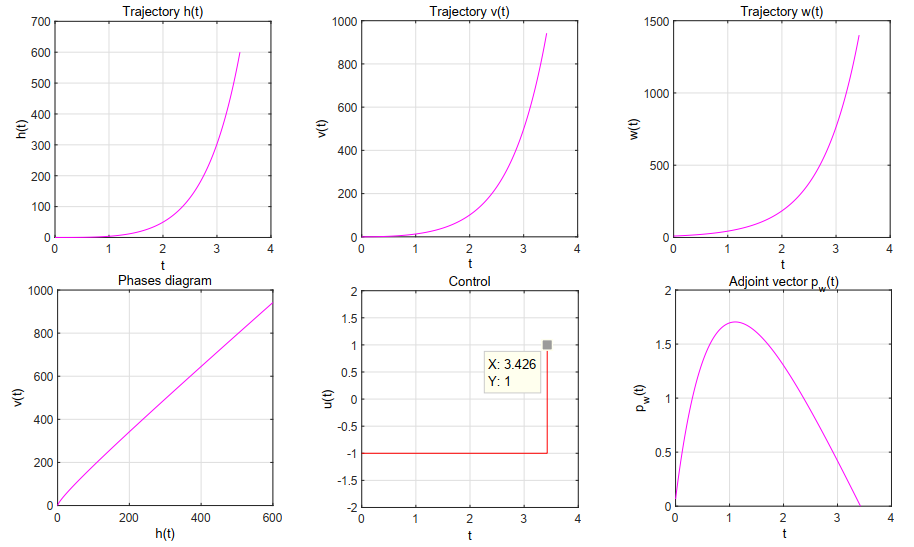
\includegraphics[scale=.6]{./image/hinh1.png}
	\caption{Kết quả của bài toán tối ưu thời gian}
\end{figure}
\\Phương pháp chụp dựa trên nguyên lý cực đại Pontryagin. Nó bao gồm việc tìm ra điểm 0 của chức năng chụp liên quan đến vấn đề thời gian tối thiểu. Đây là một phương pháp nhanh, độ chính xác cao, không yêu cầu giả định về cấu trúc điều khiển. Phương pháp chụp bao gồm ba bước chính:
\begin{itemize}
	\item \textbf{Bước 1:}
	Hình thành một bài toán giá trị biên bằng cách sử dụng các phương trình mô hình và các phương trình vectơ liền kề cũng như các điều kiện ngang.
	\item \textbf{Bước 2:}
	Xác định hàm chụp.
	\item \textbf{Bước 3:}
	Giải hệ phương trình phi tuyến.
\end{itemize}
Từ đồ thị Hình 2.1, ta suy ra $T_{\min} = 3.43s$. Biết thời gian tối thiểu này, thời gian cuối cùng của chúng ta luôn được chọn lớn hơn một chút so với $T_{\min}$. Vì vậy, chúng ta chọn $T = 3.5s$.
	\section{Bài toán vận tốc cực đại của tên lửa}
	Trong phần này, coi như thời gian cuối cùng, thời gian $T$ tìm thấy trong phần trước, tức là $T = 3.5$ giây. Đầu tiên chúng ta giải quyết vấn đề (2.4) bằng phân tích; sau đó chúng ta tiến hành phân giải số bằng 3 phương pháp: phương pháp chụp, phương pháp tùy chỉnh Cauchy và phương pháp tùy chỉnh Euler. \\
	Để giải bài toán (2.4), trước hết chúng ta áp dụng nguyên lý cực đại Pontryagin. Hàm Hamilton của
	bài toán (2.4) với $t \in [0, T]$ là
	\begin{equation}
		H(t, x(t), p(t), u(t)) = p_h(t)v(t) + p_v(t)[w(t)-g] + \alpha p_w(t)[w(t)-u(t)]
	\end{equation} Các vectơ liền kề là nghiệm của hệ sau:
\begin{eqnarray}
	\begin{cases}
		\dot{p}_h(t) = 0, \\ \dot{p}_v(t) = -p_h(t), \\ \dot{p}_w(t) = -p_v(t) - \alpha p_w(t), t \in [0, T]
	\end{cases}
\end{eqnarray}
Từ hệ thức (2.17), ta suy ra rằng
\begin{eqnarray}
	\begin{cases}
		p_h(t) = \lambda_1, \\ p_v(t) = -\lambda_1t+\lambda_2, \\ p_w(t) = \dfrac{1}{\alpha^2}(\alpha^2\lambda_3e^{-\alpha t} + \alpha\lambda_1t - \lambda_1 - \alpha\lambda_2), \\ \lambda_i \in \mathbb{R}, i = 1,2,3
	\end{cases}
\end{eqnarray} với \begin{eqnarray}
p_h(0) = \lambda_1, p_v(0) = \lambda_2, p_w(0) = \dfrac{1}{\alpha^2}(\lambda_1-\alpha\lambda_2+\alpha^2\lambda_3)
\end{eqnarray}
Cực đại hàm Halminton được cho bởi \begin{eqnarray}
	H(t, x^*(t), p^*(t), u^*(t)) &=& \max_{-1 \leq u(t) \leq 1}H(t, x(t), p(t), u(t)) \nonumber \\ &=& p_h(t)v(t) + p_v(t)[w(t)-g]\nonumber \\ &&+\alpha p_w(t)w(t) \nonumber \\&& + \alpha \max_{-1 \leq u(t) \leq 1}[-p_w(t)u(t)]. \nonumber
\end{eqnarray}
Điều khiển tối ưu Hamilton là \begin{equation}
	u^*(t) = -\text{sign}(p_w(t))
\end{equation}
Vectơ $x(T)$ phải thỏa mãn ràng buộc
$$h_1-Q'x(T)=0$$ Vì thời điểm cuối cùng $T$ là cố định trong bài toán (2.4), chúng ta nhận được các điều kiện chuyển đổi sau:
\begin{eqnarray}
	-p_h(T) - \dfrac{\partial g(x(T))}{\partial h(T)} + \dfrac{\partial(h_1 - Q'x(T))}{\partial h(T)}b = 0, \\
	-p_v(T) - \dfrac{\partial g(x(T))}{\partial v(T)} + \dfrac{\partial(h_1 - Q'x(T))}{\partial v(T)}b = 0, \\ -p_w(T) - \dfrac{\partial g(x(T))}{\partial w(T)} + \dfrac{\partial(h_1 - Q'x(T))}{\partial w(T)}b = 0,
\end{eqnarray} với $g(x(T)) = -v(T)$ và $b \in \mathbb{R}$. \\Từ đó, chúng ta có được các điều kiện biên sau: \begin{equation}
p_h(T) = -b, p_v(T) = 1, p_w(T) = 0
\end{equation}
Bằng cách sử dụng các điều kiện biên (2.24) và các mối quan hệ (2.18), chúng ta nhận được:
\begin{eqnarray}
	\begin{cases}
		p_h(t) = -b, \\ p_v(t) = b(t-T) + 1,  \\ p_w(t) = \dfrac{1}{\alpha^2}((a-b)(e^{-\alpha(t-T)} - 1) - \alpha b(t-T)),  \\ t\in[0, T].
	\end{cases}
\end{eqnarray}
	\subsection{Giải pháp phân tích}
	Vì điều khiển tối ưu bằng dấu đối nghịch của vectơ liền kề $p_w(t)$, nên thời gian giao hoán là
	được cho bởi nghiệm nguyên của phương trình $p_w(t) = 0$. Vì $A$ là ma trận bậc 3 và tất cả các giá trị riêng của $A$ là thực nên bài toán có nhiều nhất một thời gian giao hoán $t_c < T$ \\Để chọn chiến lược tối ưu, hãy xem xét các chiến lược khả thi sau:
	\begin{itemize}
		\item \textbf{Chiến lược 1} $u(t) = 1, \forall t \in [0, T]$; 
		\item \textbf{Chiến lược 2} $u(t) = -1, \forall t \in [0, T]$; \item
		\textbf{Chiến lược 3} $u(t) = 1$ với $t \in [0, t_c]$, sau đó $u(t) = -1$ với $t \in [t_c, T]$;
		\item \textbf{Chiến lược 4} $u(t) = -1$ với $t \in [0, t_c]$, sau đó $u(t) = 1$ với $t \in [t_c, T].$
	\end{itemize}

\subsubsection{Chiến lược 1}
Chúng ta có $\dot{w}(t) = \alpha[w(t) - 1]$, nghĩa là: 
\begin{eqnarray}
	\begin{cases}
		w(t) = c_1e^{\alpha t} + 1, \\ v(t) = \dfrac{c_1}{\alpha}e^{\alpha t} + (1-g)t + c_2, \\ h(t) = \dfrac{c_1}{\alpha^2}e^{\alpha t} + \dfrac{(1-g)}{2}t^2+c_2t+c_3, c_1, c_2, c_3 \in \mathbb{R}
	\end{cases}
\end{eqnarray} 
Sử dụng các điều kiện ban đầu, chúng ta thu được:
\begin{eqnarray}
	\begin{cases}
		w(t) = (g-1)e^{1.42t}+1, \\ v(t) = (g-1)\bigg(\dfrac{1}{1.42}e^{1.42t}-t-\dfrac{1}{1.42}\bigg) \\ h(t) = (g-1)\bigg(\dfrac{1}{1.42^2}e^{1.42t}-\dfrac{1}{2}t^2-\dfrac{1}{1.42}t - \dfrac{1}{1.42^2}\bigg).
	\end{cases}
\end{eqnarray}
 Với $t = T$, chúng ta sẽ có $h(T) = 549.0243 < 600.$ Do đó \textbf{Chiến lược 1} là không khả thi
 \subsubsection{Chiến lược 2} Chúng ta có $\dot{w(t)} = \alpha[w(t) + 1]$, nghĩa là: 
 \begin{eqnarray}
 	\begin{cases}
 		w(t) = d_1e^{\alpha t} - 1, \\ v(t) = \dfrac{d_1}{\alpha}e^{\alpha t} - (1+g)t + d_2, \\ h(t) = \dfrac{d_1}{\alpha^2}e^{\alpha t} - \dfrac{(1+g)}{2}t^2+d_2t+d_3, d_1, d_2, d_3 \in \mathbb{R}
 	\end{cases}
 \end{eqnarray} 
Sử dụng các điều kiện ban đầu, chúng ta thu được: 
\begin{eqnarray}
	\begin{cases}
		w(t) = (g+1)e^{1.42t}+1, \\ v(t) = (g+1)\bigg(\dfrac{1}{1.42}e^{1.42t}-t-\dfrac{1}{1.42}\bigg) \\ h(t) = (g+1)\bigg(\dfrac{1}{1.42^2}e^{1.42t}-\dfrac{1}{2}t^2-\dfrac{1}{1.42}t - \dfrac{1}{1.42^2}\bigg).
	\end{cases}
\end{eqnarray}
Với $t = T$, chúng ta sẽ có $h(T) = 673.7083 > 600$, vì vậy \textbf{Chiến lược 2} là không khả thi.

\subsubsection{Chiến lược 3}
Phương trình của tập quỹ đạo đầu tiên, khi $u(t) = 1, t \in [0, t_c]$ là: 
\begin{eqnarray}
	\begin{cases}
		w(t) = (g-1)e^{1.42t}+1, \\ v(t) = (g-1)\bigg(\dfrac{1}{1.42}e^{1.42t}-t-\dfrac{1}{1.42}\bigg) \\ h(t) = (g-1)\bigg(\dfrac{1}{1.42^2}e^{1.42t}-\dfrac{1}{2}t^2-\dfrac{1}{1.42}t - \dfrac{1}{1.42^2}\bigg).
	\end{cases}
\end{eqnarray}
Phương trình của tập quũ đạo thứ hai, khi $u(t) = -1, t\in [t_c, T]$ được cho bởi: 
\begin{eqnarray}
	\begin{cases}
		w(t) = \beta_1 e^{1.42t} + 1, \\ v(t) = \dfrac{\beta_1}{1.42}e^{1.42t} - (g+1)t+\beta_2, \\ h(t) = \dfrac{\beta_1}{1.42^2}e^{1.42t} - \dfrac{(g+1)}{2}t^2 + \beta_2t + \beta_3, \text{ }  \beta_1, \beta_2, \beta_3 \in \mathbb{R}.
	\end{cases}
\end{eqnarray}
Tại giao điểm của hai tập hợp, ta thu được: \begin{eqnarray}
	\beta_1 = (g-1) + 2e^{-1.42t_c}, \text{ } \beta_2 = 2t_c - \dfrac{(g+1)}{1.42}, \text{ } \beta_3 = -t_c^2 + \dfrac{2}{1.42}t_c - \dfrac{(g+1)}{1.42^2} \nonumber
\end{eqnarray}
Tính $t_c$ sao cho $h(T) = 600m$. Điều kiện cuối cùng này dẫn đến phương trình sau: \begin{equation}
	142.86e^{-1.42t_c} - t_c^2 + 8.41t_c - 69.15 = 0.
\end{equation}
Nghiệm số của phương trình cuối cùng này là $t_c = 0.557s.$ \\ Bằng cách thay các giá trị của $\beta_1$ và $\beta_2$ vào phương trình thứ hai của hệ (2.31), chúng ta thu được $$J(u, T) = v(T) = 940.8949\text{ }m.s^{-1}$$

\subsubsection{Chiến lược 4}
Phương trình của tập quỹ đạo đầu tiên, khi $u(t) = -1, t\in[0, t_c]$ là: \begin{eqnarray}
	\begin{cases}
		w(t) = (g+1)e^{1.42t}-1, \\ v(t) = (g+1)\bigg(\dfrac{1}{1.42}e^{1.42t}-t-\dfrac{1}{1.42}\bigg) \\ h(t) = (g+1)\bigg(\dfrac{1}{1.42^2}e^{1.42t}-\dfrac{1}{2}t^2-\dfrac{1}{1.42}t - \dfrac{1}{1.42^2}\bigg).
	\end{cases}
\end{eqnarray}
Phương trình của tập quỹ đạo thứ hai, khi $u(t) = 1, t \in[t_c, T]$ được cho bởi: \begin{eqnarray}
	\begin{cases}
		w(t) = \gamma_1e^{\alpha t} + 1, \\ v(t) = \dfrac{\gamma_1}{\alpha}e^{\alpha t} + (1-g)t + \gamma_2, \\ h(t) = \dfrac{\gamma_1}{\alpha^2}e^{\alpha t} + \dfrac{(1-g)}{2}t^2 + \gamma_2t + \gamma_3, \text{ } \gamma_1, \gamma_2, \gamma_3 \in \mathbb{R}. 
	\end{cases}
\end{eqnarray}
Tại giao điểm của hai tập hợp, ta thu được: $$\gamma_1 = (g+1) - 2e^{-1.42t_c}, \text{ } \gamma_2 = -2t_c - \dfrac{(g-1)}{1.42}, \text{ } \gamma_3=t_c^2 - \dfrac{2}{1.42}t_c-\dfrac{(g-1)}{1.42^2}.$$ Tính toán $t_c$ sao cho $h(T) = 600m$. Điều kiện cuối cùng này tạo ra phương trình sau:
\begin{equation}
	142.8555e^{-1.42t_c} + t_c^2 + 8.4085t_c + 91.8798 = 0.
\end{equation} Nghiệm số của phương trình cuối cùng này là $t_c = 0.331s$\\Theo hệ thức (2.34), giá trị mục tiêu của bài toán (2.4) bằng: $$J(u, T) = v(T) = 931.6531 \text
{ } m.s^{-1}.$$ Lưu ý rằng giá trị mục tiêu được đưa ra bởi \textbf{Chiến lược 3} cao hơn giá trị được tìm thấy trong \textbf{Chiến lược 4}, thuộc loại bang-bang. Các kết quả lý thuyết được vẽ trong Hình 2.2 và Hình 2.3.
\begin{figure}[h]
	\centering
	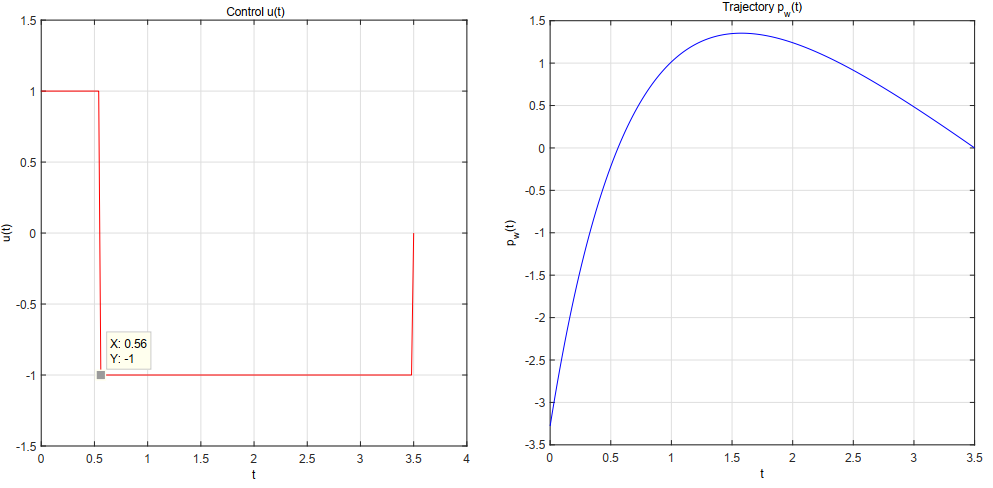
\includegraphics[scale=.6]{./image/hinh2.png}
	\caption{$t \to u(t)$ và $t \to p_w(t)$}
\end{figure}
Do đó, chúng ta đã xác định được quỹ đạo tối ưu đạt cực đại $v(T)$ và thỏa mãn điều kiện biên $h(T) = 600m$, được cho bởi
\begin{eqnarray}
u^*(t) =	\begin{cases}
		1, & t \in [0, 0.55];\\ -1, & t\in[0.55, 3.5];
	\end{cases}
\end{eqnarray} và $J(u^*, T) = v^*(T) = 940.8949 \text{ } m.s^{-1}.$

\begin{figure}[h]
	\centering
	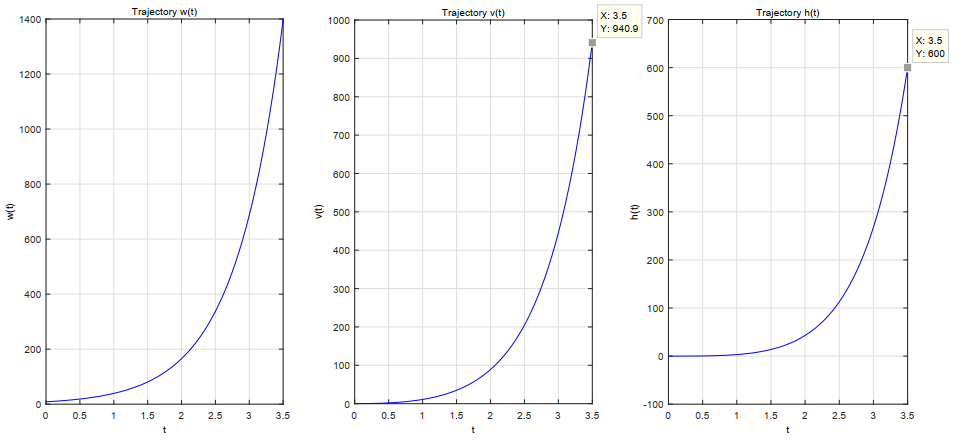
\includegraphics[scale=.6]{./image/hinh3.png}
	\caption{Quỹ đạo tối ưu $t \to h(t), t\to v(t)$ và $t\to w(t)$}
\end{figure}
	\subsection{Độ phân giải số theo phương pháp chụp}
	
	Nguyên tắc cực đại Pontryagin dẫn chúng ta đến vấn đề giá trị biên sau:
	
	\begin{eqnarray}
		\begin{cases}
			\dot{x}_1(t) = x_2(t), \\ \dot{x}_2(t) = x_3(t) - g, \\ \dot{x}_3(t) = \alpha[x_3(t) + \text{sign}(p_3(t))], \\ \dot{p}_1(t) = 0, \\ \dot{p}_2(t) = -p_1(t),\\\dot{p}_3(t) = -p_2(t) - \alpha p_3(t), \\ x_1(0) = 0, x_2(0) = 0, x_3(0)=g,\\p_1(0)=\lambda_1, p_2(0)=\lambda_2,p_3(0)=\dfrac{1}{\alpha^2}(\alpha^2\lambda_3-\lambda_1-\alpha\lambda_2),\\x_1(T)=600,x_2(T)\text{ tự do}, x_3(T)\text{ tự do}, \\p_1(T)=-b, p_2(T)=1, p_3(T)=0, 
		\end{cases}
	\end{eqnarray} với $$x(t)=(x_j(t), j=1\cdots 3) = (h(t), v(t), w(t))$$ và $$p(t) = (p_j(t), j=1\cdots 3) = (p_h(t), p_v(t), p_w(t))$$. \\Chúng ta xây dựng hàm chụp sau:
\begin{eqnarray}
	\begin{tabular}{clcl}
		$G$: & $\mathbb{R}^6$ & $\to$ & $\mathbb{R}^6$ \\
		& $(p(0), p(T))$ & $\mapsto$ & $G(p(0), p(T))$, 
	\end{tabular}
\end{eqnarray} với $$G(p(0), p(T)) = \begin{pmatrix}
p_1(0)-\lambda_1 \\ p_2(0)-\lambda_2 \\ p_3(0) - \dfrac{1}{\alpha^2}(\alpha^2\lambda_3 - \lambda_1-\alpha\lambda_2)\\p_1(T)+b\\p_2(T)-1\\p_3(T)-0
\end{pmatrix}.$$

Do đó, bài toán (2.37) tương đương với bài toán sau:
\begin{eqnarray}
	\begin{cases}
	\dot{x}_1(t) = x_2(t), \\ \dot{x}_2(t) = x_3(t)-g, \\ \dot{x}_3(t) = \alpha[x_3(t)+\text{sign}(p_3(t))], \\ \dot{p}_1(t) = 0, \\\dot{p}_2(t) = -p_1(t), \\ \dot{p}_3(t) = -p_2(t)-\alpha p_3(t), \\x_1(0)=0,x_2(0)=0,x_3(0)=g, \\ x_1(T)=h_1, x_2(T) \text{  tự do}, x_3(T) \text{ tự do}, \\ G(p(0), p(T)) = 0.
\end{cases}
\end{eqnarray}
Ta xác định nghiệm số của hệ phi tuyến $G(p(0), p(T)) = 0$ bằng phương pháp Newton. Bằng cách thực hiện phương pháp này với Matlab, chúng ta tìm thấy kết quả được vẽ trong Hình 2.4. \\ Kết quả này cho thấy thời gian giao hoán là $t_c = 0.557s$, vận tốc cực đại là $v^*(T) = 940.8949 m.s^{-1}$. Thời gian thực hiện của phương pháp chụp là $t = 1.9781s$. Chúng ta nhận xét rằng phương pháp chụp đã cho kết quả tương tự như phương pháp phân tích trong thời gian CPU ngắn. Điều này cho thấy phương pháp chụp nhanh và cho kết quả chính xác đối với vấn đề được nghiên cứu.
\begin{figure}[h]
	\centering
	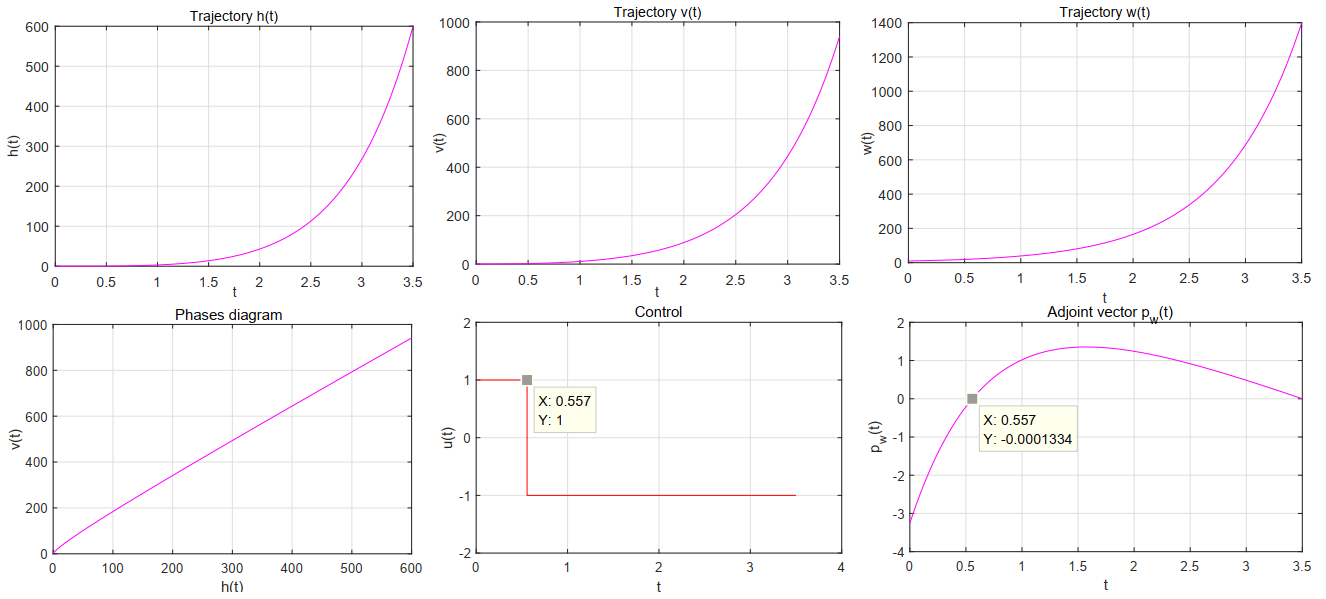
\includegraphics[scale=.45]{./image/hinh4.png}
	\caption{Kết quả số của phương pháp chụp}
\end{figure}

	\subsection{Độ phân giải số theo phương pháp tùy chỉnh Cauchy}
	Đối với một số khoảng thời gian con tùy chỉnh $N$ được chọn trước, bước tùy chỉnh là $\theta = \dfrac{T}{N}$\\
	Nghiệm của hệ động lực học của bài toán (2.4) được cho bởi:
	\begin{equation}
		x(t) = F(t)x_0 + \int_{0}^{t}F(t)(F(s))^{-1}[Bu(s)+r(s)]ds, t \in [0, T],
	\end{equation} trong đó $F(t)$ là một hàm số, là nghiệm của hệ thống sau:
	$$\dot{F}(t) = AF(t), F(0)=I_3, t \in[0, T].$$ Sử dụng giải pháp cuối cùng này, vấn đề ban đầu (2.4) có dạng sau:
	\begin{equation}
		\begin{cases}
			\max_{u(t)} J(u(t)) = c^{'}F(T)x_0 + \int_{0}^{T}\psi(t)dt + \int_{0}^{T}C(t)u(t)dt, \\ \int_{0}^{T}\varphi(t)u(t)dt = \bar{g} \\ -1 \leq u(t) \leq 1, t \in [0, T],
		\end{cases}
	\end{equation} với $$
	C(t) = c'F(T)F(t)^{-1}B, \varphi(t) = Q'F(T)F(t)^{-1}B,  $$ $$\psi(t) = c'F(T)F(t)^{-1}r, $$$$ \bar{g} = h_1 - Q'F(T)x_0 - \int_{o}^{T}Q'F(T)F(t)^{-1}rdt.
$$ Cho $\tau^j = \tau_{j+1} = \tau_j + \theta$, do đó ta có $$[0, T] = \cup_{j=1}^{N-1}[\tau_j, \tau^j]\cup[\tau_N, \tau^N].$$ Chúng ta tính các giá trị $C_j, X_j$ như sau: 
$$C_j = \int_{\tau_j}^{\tau^j}C(t)dt,$$$$X_j = \int_{\tau_j}^{\tau^j}\varphi(t)dt, \psi_j=\int_{\tau_j}^{\tau^j}\psi(t)dt$$$$\bar{g}_j=h_1 - Q'F(T)x_0 - \int_{\tau_j}^{\tau^j}Q'F(T)F(t)^{-1}rdt, j = 1, \cdots, N.$$ Do đó, chúng ta nhận được bài toán lập trình tuyến tính sau: 
\begin{equation}
	\begin{cases}
		\max_u J(u) = \Sigma_{j=1}^{N}C_ju_j, \\\Sigma_{j=1}^{N}X_ju_j = \bar{g}, \\ -1 \leq u_j \leq 1, j = 1, \cdots N.
	\end{cases}
\end{equation}
Chúng tôi đã giải quyết chương trình tuyến tính này cho các giá trị khác nhau của $N$ bằng phương pháp điểm bên trong được triển khai trong MATLAB2009b được thực thi với PC có bộ vi xử lý Core i5, 2.40Ghz và RAM 6 GO. Thời gian thực hiện của thuật toán tùy biến Cauchy $T_1$, số lần lặp $Nit$ và thời gian thực hiện $T_2$ của bộ giải điểm bên trong, tổng thời gian thực hiện $T = T_1 + T_2$, cũng như tốc độ tối đa tại thời điểm cuối cùng $v(T)$ đối với các giá trị khác nhau của $N$, được trình bày trong Bảng 2.1.

\begin{table}[!htp]
	\centering
	\begin{tabular}{|c|c|l|l|c|l|}
		\hline
		$N$ & $v(T)$ & $Nit$ & $T_1(s)$ & $T_2(s)$ & $T(s)$ \\
		\hline
		10 & 940.7414 & 6 & 5.9679 & 0.2645 & 6.2342 \\
		\hline
		50 & 940.8939 & 8 & 21.1047 & 0.2557 & 21.3604 \\
		\hline
		100 & 940.8944 & 8 & 41.5202 & 0.2535 & 41.7788 \\
		\hline
		150 & 940.8946 & 8 & 62.7943 & 0.2584 & 62.0527 \\
		\hline
		200 & 940.8947 & 8 & 78.0943 & 0.2656 & 78.3599 \\
		\hline
		500 & 940.8948 & 8 & 228.3542 & 0.2671 & 228.6218 \\
		\hline
		800 & 940.8948 & 9 & 421.2051 & 0.2825 & 421.4875 \\
		\hline
		900 & 940.8949 & 9 & 505.9931 & 0.3897 & 506.3828 \\
		\hline
		1000 & 940.8949 & 9 & 544.6023 & 0.4282 & 545.0209 \\
		\hline
		2000 & 940.8949 & 10 & 1584.1246 & 0.2918 & 1584.4317 \\
		\hline
	\end{tabular}
\caption{Kết quả mô phỏng số cho phương pháp tùy chỉnh Cauchy}
\end{table} 
\noindent Chúng ta nhận xét rằng kỹ thuật điều chỉnh Cauchy đã tìm ra giải pháp tối ưu được tính toán phân tích với 2 số thập phân chính xác trong 21.36 giây và với 4 số thập phân chính xác trong 506.38 giây. Điều này cho thấy phương pháp này có thể cho kết quả chính xác nhưng trong khoảng thời gian lớn.

	\subsection{Độ phân giải số bằng phương pháp tùy biến Euler}
	Đối với một số khoảng thời gian con $N$ được chọn trước, chúng ta sẽ có bước tùy biến $\theta = \dfrac{T}{N}$ và thời gian như sau: $$0 = t_0 < t_1 < \cdots < t_{N-1} < t_N = T.$$
	Việc áp dụng sơ đồ tùy biến Euler để giải các bài toán giá trị biên cho chúng ta bài toán lập trình tuyến tính sau:
	\begin{eqnarray}
		\begin{cases}
			\text{Maximize } J(u, T) = v(T), \\ h(t_{i+1}) = h(t_i) + \theta v(t_i), & i = 0,1,\cdots, N, \\ v(t_{i+1}) = v(t_i) + \theta[w(t_i) - g], & i=0,1,\cdots, N, \\ w(t_{i+1}) = w(t_i) + \alpha\theta[w(t_i) - u(t_i)],& i = 0,1,\cdots, N, \\ h(0) = 0, v(0) = 0, w(0) = g, h(t_N) = 600. 
		\end{cases}
	\end{eqnarray}
	Chúng ta cũng đã giải quyết chương trình tuyến tính (2.43) bằng bộ giải điểm bên trong của MATLAB2009b. Các kết quả thu được (thời gian thực hiện phương pháp điểm trong $T$, số lần lặp $Nit$ và tốc độ lớn nhất $v(T)$) được trình bày trong Bảng 2.2.
	\begin{table}[!thp]
		\centering
	\begin{tabular}{|l|l|c|c|}
		\hline
		$N$ & $v(T)$ & $Nit$ & $T(s)$ \\
		\hline
		200 & 943.7800 & 12 & 0.0092 \\
		\hline
		500 & 942.2125 & 12 & 0.0464 \\
		\hline
		800 & 941.7509 & 11 & 0.1007 \\
		\hline
		1200 & 941.4787 & 11 & 0.1726 \\
		\hline
		2000 & 941.2552 & 31 & 1.6544 \\
		\hline
		3000 & 941.1352 & 25 & 1.5569 \\
		\hline
	\end{tabular}
\caption{Kết quả mô phỏng số cho phương pháp tùy biến Euler}
	\end{table} \\
Từ Bảng 2.2, chúng ta có thể nhận xét rằng phương pháp tùy chỉnh Euler rất nhanh, tuy nhiên ngay cả với bước tùy chỉnh lớn, nó vẫn không thể đạt được độ chính xác mong muốn.
	\subsection{So sánh số}
	Tốc độ tối ưu được tìm thấy bởi bốn phương pháp gần như tương tự nhau, tuy nhiên thời gian thực hiện của các phương pháp này khá khác nhau. Lưu ý rằng phương pháp chụp cho tốc độ tối ưu với độ chính xác cao và yêu cầu thời gian thực hiện rất ngắn (1.97 giây). Đối với $N = 900$, phương pháp tùy biến Cauchy cho vận tốc tối đa với độ chính xác 4 số thập phân với thời gian thực hiện là 506.38 giây, trong khi phương pháp tùy chỉnh Euler cho $N = 3000$ một tốc độ tối ưu với sai số bằng 0.34 và thời gian thực hiện trong 1.55 giây. Điều này cho thấy rằng: 
	\begin{itemize}
		\item Phương pháp chụp có độ chính xác cao và nhanh chóng
		\item Phương pháp tùy biến Cauchy có độ chính xác cao nhưng chậm.
		\item Phương pháp tùy biến Euler rất nhanh nhưng kém chính xác hơn các phương pháp khác.
	\end{itemize}
\begin{figure}[h]
	\centering
	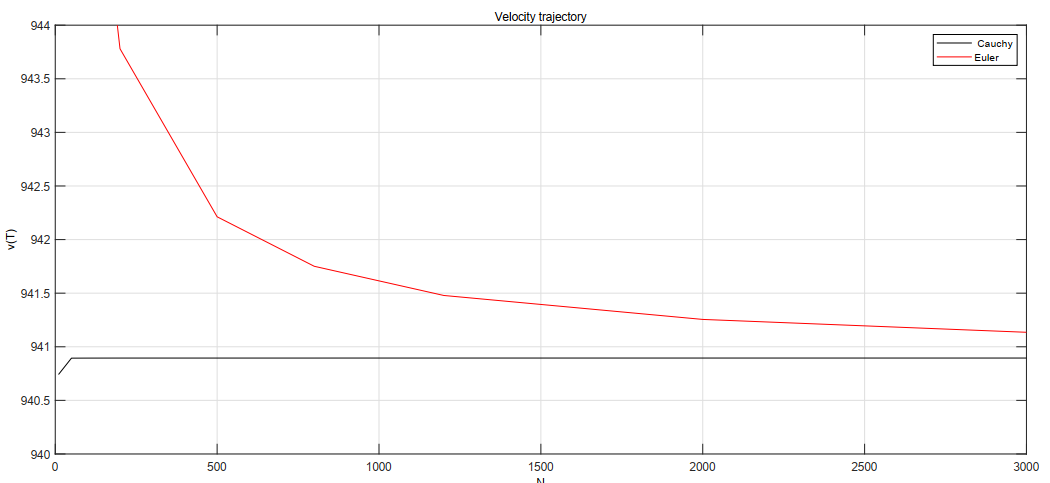
\includegraphics[scale=.55]{./image/hinh5}
	\caption{So sánh số của các phương pháp số khác nhau}
\end{figure}
	\chapter{Kết luận}
	Trong đồ án này, chúng ta đã giải quyết một vấn đề thực tế phát sinh trong lĩnh vực hàng không vũ trụ bằng cách xây dựng nó như một bài toán điều khiển tối ưu tuyến tính. \\ Đối với độ phân giải lý thuyết, nguyên tắc tối đa Pontryagin đã được sử dụng để đưa ra điều kiện tối ưu cần thiết. Về mặt số học, vấn đề được xem xét được giải quyết bằng phương pháp chụp và hai kỹ thuật tùy biến (kỹ thuật sử dụng công thức Cauchy và một kỹ thuật sử dụng công thức Euler). Các giải pháp tối ưu thu được gần như tương tự nhau, nhưng có sự khác biệt lớn về thời gian thực hiện của ba phương pháp số. \\ Hướng nghiên cứu mở rộng tiếp theo là thêm một tham số mới (góc gót chân) và các ràng buộc khác, sau đó mô hình chuyển động của tên lửa như một bài toán điều khiển tối ưu phi tuyến.
	
\end{document}